\documentclass[tikz,border=6mm]{standalone}

\usepackage[T1]{fontenc}
\usepackage[scaled=0.92]{helvet}
\renewcommand{\familydefault}{\sfdefault}

\usepackage{tikz}
\usetikzlibrary{positioning,calc,arrows.meta}

\begin{document}

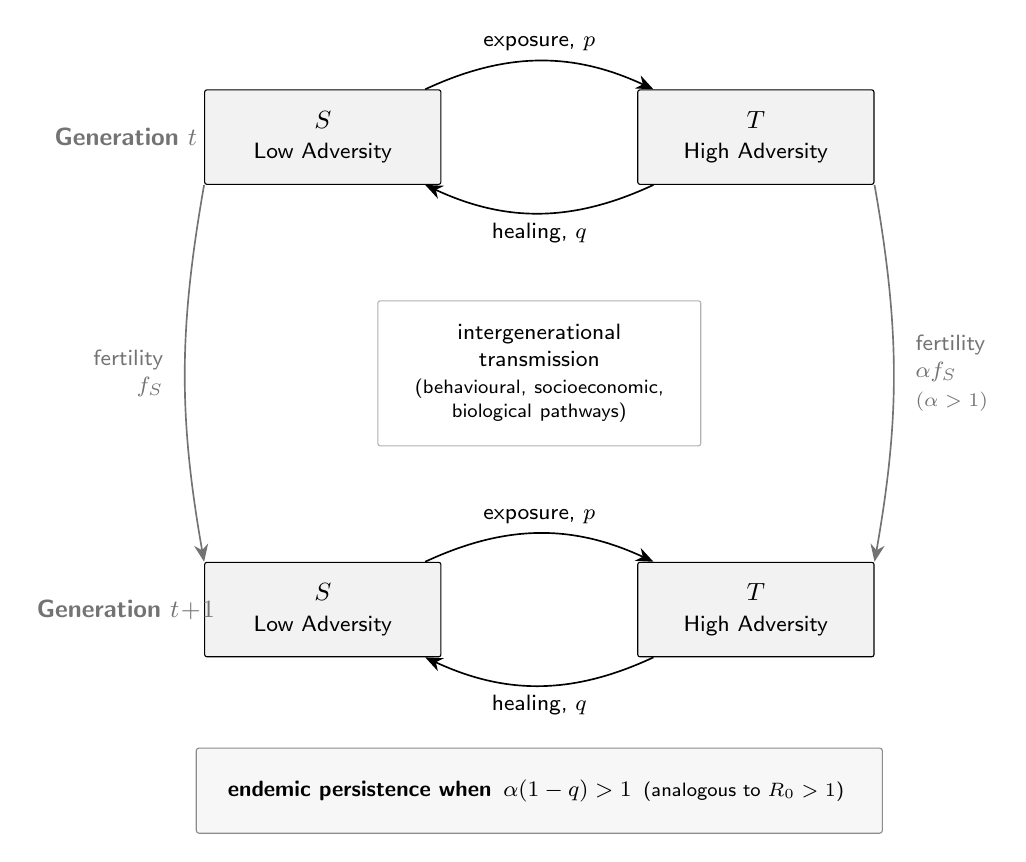
\begin{tikzpicture}[
  state/.style={
    draw, rounded corners=0.8pt, fill=gray!10,
    minimum width=3cm, minimum height=1.2cm,
    align=center, font=\small
  },
  arr/.style={-{Stealth[length=2.2mm,width=1.8mm]}, semithick},
  repr/.style={-{Stealth[length=2.2mm,width=1.8mm]}, semithick, black!55},
  lbl/.style={font=\footnotesize},
  genlbl/.style={font=\small\bfseries, text=black!55},
]

%% --- Generation t ---------------------------------------------------
\node[state] (St)  at (0,   0) {$S$\\\footnotesize Low Adversity};
\node[state] (Tt)  at (5.5, 0) {$T$\\\footnotesize High Adversity};

\draw[arr, bend left=25] (St) to node[above, lbl]{exposure,~$p$} (Tt);
\draw[arr, bend left=25] (Tt) to node[below, lbl]{healing,~$q$}  (St);

\node[genlbl] at (-2.5, 0) {Generation $t$};

%% --- Generation t+1 ------------------------------------------------
\node[state] (St1) at (0,   -6) {$S$\\\footnotesize Low Adversity};
\node[state] (Tt1) at (5.5, -6) {$T$\\\footnotesize High Adversity};

\draw[arr, bend left=25] (St1) to node[above, lbl]{exposure,~$p$} (Tt1);
\draw[arr, bend left=25] (Tt1) to node[below, lbl]{healing,~$q$}  (St1);

\node[genlbl] at (-2.5, -6) {Generation $t\!+\!1$};

%% --- Reproduction arrows (outer edges, clear of center) ------------
%  Left: route along the west side of the S nodes
\draw[repr, out=260, in=100]
  (St.south west) to
  node[left=1.5mm, lbl, align=right]{fertility\\$f_S$}
  (St1.north west);

%  Right: route along the east side of the T nodes
\draw[repr, out=280, in=80]
  (Tt.south east) to
  node[right=1.5mm, lbl, align=left]{fertility\\$\alpha f_S$\\[1pt]\scriptsize$(\alpha>1)$}
  (Tt1.north east);

%% --- Central intergenerational label (width-constrained) -----------
\node[
  draw=black!30, rounded corners=0.8pt, fill=white,
  align=center, inner sep=3mm, font=\footnotesize,
  text width=3.5cm
] at (2.75, -3) {
  intergenerational\\transmission\\[2pt]
  \scriptsize(behavioural, socioeconomic,\\[-1pt]\scriptsize biological pathways)
};

%% --- Persistence threshold box (below) -----------------------------
\node[
  draw=black!45, rounded corners=1pt, fill=gray!6,
  align=center, inner sep=4mm, font=\footnotesize
] at (2.75, -8.3) {
  \textbf{endemic persistence when}\enspace
  $\alpha(1-q)>1$\enspace
  \scriptsize(analogous to $R_0>1$)
};

\end{tikzpicture}

\end{document}
